\documentclass[../main.tex]{subfiles}
\begin{document}

\chapter{Seminal work: TWAS from individual-level data}
\labch{gamazon2015}

\begin{external_abstract}{title=Abstract}
Genome-wide association studies (GWAS) have identified thousands of 
variants robustly associated with complex traits. However, the 
biological mechanisms underlying these associations are, in general, not 
well understood. We propose a gene-based association method called 
PrediXcan that directly tests the molecular mechanisms through which 
genetic variation affects phenotype. The approach estimates the 
component of gene expression determined by an individual's genetic 
profile and correlates 'imputed' gene expression with the phenotype 
under investigation to identify genes involved in the etiology of the 
phenotype. Genetically regulated gene expression is estimated using 
whole-genome tissue-dependent prediction models trained with reference 
transcriptome data sets. PrediXcan enjoys the benefits of gene-based 
approaches such as reduced multiple-testing burden and a principled 
approach to the design of follow-up experiments. Our results demonstrate 
that PrediXcan can detect known and new genes associated with disease 
traits and provide insights into the mechanism of these associations.
\end{external_abstract}

\section{Introduction}

Albeit it is accepted that in the majority of cases the biological role 
of variants associated to diseases is regulatory, as confirmed by the 
fact that many such variants fall in regions that are epigenetically 
marked as regulatory, GWAS results remain mainly uncharacterised from a 
functional point of view, and are only able to explain a little 
proportion of phenotypic variance. The wealth of biological data that is 
now being released by large-scale consortia provides an unprecedented 
opportunity to integrate information and obtain insight into the genetic 
and biological processes underlying disease susceptibility; some of 
these consortia, whose datasets have been exploited by Gamazon \etal, 
are as follows.

\begin{description}
	\item[GTEx Project.] Its aim is to collect data on genotype and gene 
		expression levels of a number of tissues from postmortem 
		samples.
	\item[ENCODE.] The focus is on the systematic functional annotation 
		of each segment of the human genome.
	\item[GEUVADIS.] This projects
	\item[DGN.]
	\item[Braineac.]
\end{description}

\section{The imputation of gene expression}

first step: gene expression is decomposable in three components: genetically
regulated expression (GReX), phenotype-influenced expression, and an
environmental component. The phenotype can influence gene expression.

An additive model trained on reference transcriptome datasets finds for each
SNP the coefficents of which gene expression is altered by that SNP, \ie 
it
says that SNP rs483920482905, when present in an individual, alters the
expression of gene XXXX by a factor 1.5. Clearly, the training dataset must
contain both genome and transcriptome data. Afterwards, the GReX is predicted
in indivuduals for which only the genome sequence is available.

---------

append this to "although...": The use of multiple linear regression, 
though a simplistic approach, is however a first attempt to 
quantitatively model the interactions among genetic variants: indeed, it 
may well be that a given phenotype is influenced by a 
\textit{combination} of SNPs rather than a single SNP.

They thus generated predictDB, which stores the coefficients of which 
each SNP influence the GReX. By using healthy individuals from reference 
transcriptome and genome data sets, they disregard the 
disease-determined component of gene expression, and by using a 
regression model, they disregard the random environmental component. It 
is now possible to \enquote{impute} the transcriptome of an individual 
from its genotype, just like it has been possible to impute unknown 
variants in an individual from its known genotyped variants.

\begin{figure}
	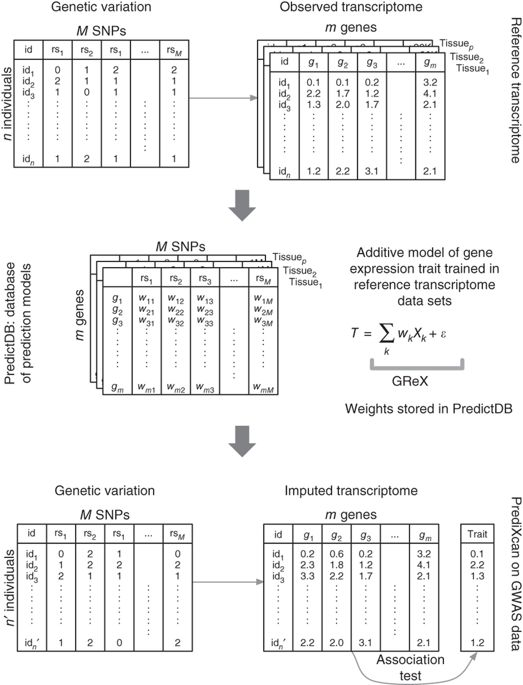
\includegraphics{gamazon2015/2-grex_estimation}
	\labfig{gamazon2015/2}
	\caption{The framework to estimate the coefficient by which each SNP 
		alters the expression of a gene.}
\end{figure}

The regression model employed can be summarised with the following 
equation (referring to \reffig{gamazon2015/2}):

\begin{equation}
	T = \sum_{k=1}^{M}{w_k X_k + \epsilon}
\end{equation}

where T is the expression of a gene, $w_k$ is the weigth of SNP $k$ in 
influencing the expression of that gene, and $X_k$ is the number of 
reference alleles of SNP $k$ in all the dataset. To fit this model, the 
authors tried various types of regression methods ---lasso, elastic net 
and \todo{another}---, but finally settled to elastic net (with the 
parameter $\alpha = 0.5$), whose main advantage is the 
\enquote{automatic} selection of the most important regressors. In 
general elastic net is used for two reasons: first, when the number of 
predictors is large, especially if compared to the number of samples; 
and second, to avoid overfitting.

They chose to use elastic net and used tenfold cross-validation (\ie 
they looked at the R square of estimated GReX vs observed expression).

\section{The correlation between expression and phenotype}

In the second phase, the predicted $\hat{GReX}$ is correlated with the 
phenotypic status employing linear regression, logistic regression, Cox 
regression, or Spearman correlation (the latter is non-parametric). They 
chose to use logistic regression for the results discussed in this 
article. Another possibility could have been that to model not the 
disease status, which is a binary variable, but rather the liability to 
the disease, following what Vissher\cite{Visscher2008} reported, showing 
that this approach is able to explain a larger proportion of genetic 
variance.

\section{PrediXcan: pros and cons}

Main advantages:

\begin{itemize}
\item directionality, possibility to get insights on mechanisms.
\item small multiple-testing burden.
\item possibility form functional units (e.g. basing on known pathways).
\item possibility to reanalise gwas data (only the genome is needed).
\end{itemize}

%\section{Prereq: 
%https://www.sciencedirect.com/science/article/pii/S0002929710005987?via%3Dihub}

%\subsection{pre-prereq: https://www.nature.com/articles/nature08494}

limits: there is an attenuation bias because of the error in the 
estimation of the GReX.



\section{Predicting the transcriptome}

They also computed the heritability of gene expression in DGN and claim 
that heritability \marginnote{Heritability is defined as the proportion 
	of phenotypic variance that is due to genetic variance} is an upper 
bound to how well the trait can be associated to the genotype. This 
makes sense, because if the variance in a trait is entirely due to the 
environment, the association study will not find anything.

The average heritability calculated in DGN was 0.153, while the average 
tenfold cross-validated prediction $R^2$ value for elastic net was 
0.137, so: not bad. Does this make sense? I think so, because 
  heritability can be interpreted as the slope of the line of the 
predicted variable as a function of the predictor (\eg offspring height 
as a function of parent height). In this case the "predictor" is the 
phenotype of the training sample, and the "predicted" is the phenotype 
in the testing sample. A high heritability says that parent height can 
predict offspring height, and that this predictability is due to genetic 
factors; here, the authors are trying to predict a phenotype (gene 
expression, but it is hardly relevant) from a genotype, which in turn 
was attributed scores according to the phenotype. The linear model 
(actually elastic net) they made, mimics the actual process of 
development: they go from one genotype to a phenotype, attributing to 
each element of the genotype (\ie to each SNP) a coefficient that 
measures how much that element is involved in the manifestation of that 
phenotype. Then, let us imagine that the training people have offspring, 
and that the offspring is the "testing people": many of the SNPs will be 
transmitted from parents to offspring. offspring have a similar genotype 
to their parents (abstracting things, offspring are merely people which 
have a genome similar to their parents), but do they have also a similar 
phenotype? If the trait is heritable, yes. In yet other words, if the 
trait is heritable, people with a similar genotype (\ie relatives) will 
have a similar phenotype (h2 is precisely the correlation between the 
phenotypes in parents-offspring); in a sense, in this paper the testing 
people (those in the gwas) are relatives of the training people (those 
in the reference transcriptome study like GEUVADIS). All this is 
expressed in figure 3.

An important thing that perhaps I did not say before is that previously 
they had imputed the SNPs of the DGN people. They used both 1000 Genomes 
and HapMap Phase 2 to impute, and achieved similar results, therefore 
they chose to restrict the imputation to hapmap to save computation 
time.

They then tested their models to see wether, given a genotype, they 
could predict the expression. That is to say, they predicted expression 
from a set of genotypes and then confronted it with the real expression. 
They used GEUVADIS and GTEx as tests. In figure 4 they show that the 
correlation between predicted and actual expression in this separate 
cohort is very different from the expected correlation under the 
hypothesis that the two vectors (predicted and actual expression) are 
independent. In gray there is a 45-degree line: if the point lay on this 
line, then on the two axes there are identical variables. on the y axis 
there are the quantiles of observed R2 (a quantile is the percentage of 
points below a given value), while on the x axis there are the quantiles 
of expected R2. A point is produced when the two quantiles are equal. 
For instance, if the 10th quantile in the observed R squareds have an R2 
of 0.2, what is the R2 of the expected R2 at the 10th quantile? In other 
words, the curve is parametric. This Q-Q plot is used to check whether 
two populations are similar.

They also note that the same situation arises for different tissues.

In fig 5 they present some example genes.

they also made a linear model for trans eQTL, with linear regression, 
but it had a poorer predictive power, so they resolved to use local SNPs 
only.

\section{Application of PrediXcan to WTCCC}

At last, they apply their method. they used DGN whole-blod elastic net 
prediction models to predict the expression in the WTCCC cohort, then 
correlated the predicted GReX with the disease status.

An interesting consideration (by fmarotta) is that many of the genes 
that were associated to the disease status were in the HLA or MHC 
region; also, the most significant results were for autoimmune diseases 
(this can be due to the fact that also in the WTCCC work the most 
significant results were for autoimmune diseases. Nay, I think that the 
fact that the two studies (WTCCC and gamazon) have found the same result 
is due to a common underlying cause, which is the same for which most 
GWAS hits are in the MHC region.) Think more about this.

They made a manhattan plot and another quantile-quantile plot. Also a 
gwas enrichment.

Some genes were associated with multiple autoimmune disease. Question by 
fmarotta: what determines which disease you have if the expression of 
that gene is altered in you? environment? gene expression level? Anyway, 
this is an example of the complexity of the situation: the relationship 
between genotype and phenotype is not biunivocal at all. the authors say 
that lower expression of dclre1b was associated with rheumatoid 
arthritis and T1D, whereas higher expression with crohn's disease.

An advantage of predicscan is that it provides directionality: we know 
if higher or lower expression is associated with the disease. See the 
example of ERBB3.

Globally, many genes were previously reported or fell near reported 
genes. Or: they were in the MHC.

Using less stringent significance thresholds, they found the same high 
enrichments of reported genes among the results of predicscan. This 
suggests that there are many false-negatives at the higher thresholds. 
The method is not so powerful afterall. They found also two completely 
novel genes.

Finally, they compared their method with two other gene-based tests: 
vegas and skat. In the quantile-quantile plot, predixcan was the best in 
the tail-end.

\section{Discussion}

Why gene expression? It is the most direct phenotype (indeed, sometimes 
we speak about \enquote{extended phenotypes}; gene expression can also 
be viewed as an intermediate phenotype), it is heritable, and virtually 
all the other phenotypes depend on it. Moreover, it is easy to measure.

fmarotta:Genes can do few things: either they bind proteins whith a 
structural or regulatory function (and when it is structural, it can be 
regulating: TAD are coregulated), or they are transcribed, starting a 
series of biochemical reactions that ultimately lead to functional 
molecules, be they RNA or proteins. The complexity stems from the 
interactions of many genes together and with the environment

Limits:
\begin{itemize}
	\item
the prediction of gene expression can be biased, and some models, namely 
a combination of K nearest neighbour (KNN), elastic net, and the use of 
genomic annotation may perform better.
	\item 
(https://www.cell.com/ajhg/fulltext/S0002-9297(18)30108-3?code=cell-site) 
Genetic variation does not alter only gene expression. There can be 
\textit{trans}-acting effects, where a SNP alters how a gene (be it a TF 
or a miRNA) modulates the expression of others, without altering the 
expression of the modulator gene itself. Moreover, a SNP can have 
effects on splicing, transcription start or end site or other RNA 
editing processes, without altering the expression of the gene.
\end{itemize}

One of the main advantages is that it is economic: one only needs 
existing data, therefore many existing GWAS dataset can be reanalysed 
\enquote{for free}.

Another virtue is that predicscan provides directionality, hinting at 
potential strategies to cure disease, \eg if a gene's upregulation is 
linked to a disease, then a drug may be developed to downregulate it. 
(by fmarotta: It probably woul have no effect whatsoever because of 
compensatory effects.)

Multiple testing: here they have used bonferroni, which is pretty 
conservative. They only corrected gene-based tests of association, and 
not SNP-based ones, because the gene-based association is the last step, 
and because bonferroni is conservative. (by SNP-based, I do not know if 
they mean SNP-geneexpression association or SNP-trait association 
performed in a classical GWAS.)

They do not claim causality, for SNPs may contribute both to expression 
and to other things, and it may be that the other things are the cause 
of the disease, not gene expression.

They state that their method provides insights into gene regulation and 
directionality.

by fmarotta: Actually, they do not prove that a SNP associated to gene 
expression regulates the gene: they  only say that variation between 
individuals at that locus results in variation in gene expression. Or do 
they?

\end{document}
